\documentclass{article}
\usepackage{arxiv}
\usepackage{amsmath,amssymb,amsthm}
\usepackage{graphicx}
\usepackage{booktabs}
\usepackage[hypertexnames=false]{hyperref}
\usepackage{xcolor}
\usepackage{natbib}
\usepackage{algorithm}
\usepackage{algorithmic}

\newtheorem{remark}{Remark}

\renewcommand{\shorttitle}{AD-IRT-Mem: Psychometric Token Allocation for OCR-Memory}

\hypersetup{
  colorlinks=true,linkcolor=black,citecolor=black,urlcolor=blue,
  pdftitle={AD-IRT-Mem: Psychometric Token Allocation for OCR-Memory Systems},
  pdfauthor={Jung Min Kang},
  pdfsubject={Item Response Theory, OCR-Memory, Token Allocation},
  pdfkeywords={IRT, OCR-Memory, Fisher Information, agent memory}
}

\title{AD-IRT-Mem: Psychometric Token Allocation\\for OCR-Memory Systems}
\author{
  Jung Min Kang \\
  Independent Researcher, Seoul, South Korea \\
  \texttt{gangjeongmin23@gmail.com}\ \ ORCID: 0009-0007-9599-2792
}
\date{May 2026}

\begin{document}
\maketitle

\begin{abstract}
OCR-Memory systems store agent histories as images for token-efficient retrieval, but lack principled criteria for resolution allocation across memory chunks. We introduce AD-IRT-Mem, a framework mapping OCR-Memory token budgeting onto Computerized Adaptive Testing via Item Response Theory (IRT): chunks are items with latent difficulty, queries are subjects with latent ability, and Fisher Information weights resolution allocation. On synthetic data (480~chunks, 80~queries, disjoint train/CV/eval splits, 5~seeds), we establish three results. First, AD-IRT-Mem achieves 98.4\% win rate over greedy top-$k$ allocation ($\Delta\mathrm{IRR} = +0.057$), establishing that concentrated resolution is a systematic failure mode. Second, uniform allocation beats AD-IRT-Mem in 80\% of conditions; we show this follows from the concavity structure of OCR accuracy functions, where the optimal budget distribution equalizes marginal returns across chunks---a condition that retrieval pre-filtering approximately satisfies. Third, the LLTM decomposes chunk difficulty into observable features with perfect weight ranking recovery ($\rho = 1.0$). These results provide a novel framework for OCR-Memory token budgeting and a theoretical characterization of when principled allocation can and cannot outperform uniform distribution.
\end{abstract}

\noindent\textbf{Keywords:} Item Response Theory, OCR-Memory, token allocation, Fisher Information, agent memory

\section{Introduction}

Autonomous LLM agents increasingly operate in long-horizon settings where success depends on reusing experience from extended histories~\citep{li2026ocr,feng2026agentocr}. OCR-Memory~\citep{li2026ocr} and related frameworks~\citep{shi2026memocr,feng2026agentocr} address the token budget bottleneck by encoding trajectories as images, exploiting visual token density. DeepSeek-OCR~\citep{wei2025deepseekocr} achieves approximately 97\% OCR precision below $10\times$ compression.

A fundamental question remains: given a fixed token budget, how should resolution be allocated across candidate memory chunks? Current systems allocate uniformly, use recency heuristics, or train RL policies~\citep{shi2026memocr}. We propose a psychometric formulation and find that the answer is more nuanced than ``use IRT.''

\paragraph{Contributions.}
\begin{enumerate}
\item To our knowledge, the first structural mapping between Computerized Adaptive Testing (CAT) and OCR-Memory token allocation (Table~\ref{tab:iso}).
\item An analysis showing that concavity of OCR accuracy functions explains uniform allocation's strength via a marginal-return equalization argument (Remark~\ref{rem:concavity}).
\item AD-IRT-Mem: Fisher-Information-weighted allocation that prevents the top-$k$ failure mode (98.4\% win rate, $\Delta = +0.057$).
\item LLTM cold-start: observable chunk features predict difficulty with perfect ranking recovery ($\rho = 1.0$).
\end{enumerate}

\section{Background and Isomorphism}

\subsection{OCR-Memory Systems}

OCR-Memory~\citep{li2026ocr} stores trajectories as images with visual anchors and retrieves via locate-and-transcribe. AgentOCR~\citep{feng2026agentocr} achieves over 95\% task performance at over 50\% token reduction. MemOCR~\citep{shi2026memocr} uses layout-aware visual memory with RL-based budget optimization. In the broader vision-transformer literature, ARTA~\citep{hagerman2026arta} uses adaptive mixed-resolution token allocation for dense feature extraction, allocating fine tokens to semantically complex regions; our work differs by introducing a psychometric allocation model for OCR-memory chunks. At the core is a budget allocation problem: maximizing task-relevant information within limited tokens~\citep{shi2026memocr}.

\subsection{IRT for AI Evaluation}

The Evaluation Failure Scaling Law (EFSL)~\citep{kang2026efsl} showed that IRT maintains $\rho \geq 0.993$ where averaging degrades to $\rho = 0.24$ under biased missingness. AD-IRT~\citep{kang2026adirt} blends IRT and MIRT via coverage-breadth modulation. PCR~\citep{kang2026pcr} uses the frontier value $\mathcal{F} = P(1-P)$ for content routing. IRT-Router~\citep{song2025irt} applies IRT for multi-LLM routing.

\subsection{The Structural Isomorphism}

\begin{table}[ht!]
\centering
\caption{Structural isomorphism between CAT and OCR-Memory allocation.}
\label{tab:iso}
\begin{tabular}{ll}
\toprule
\textbf{CAT Concept} & \textbf{OCR-Memory Analog} \\
\midrule
Item difficulty $b_j$ & Chunk information density \\
Subject ability $\theta_i$ & Query specificity \\
Item discrimination $a_j$ & Chunk retrieval sensitivity \\
Test length budget & Token budget $B$ \\
Fisher Information $I(\theta)$ & Resolution allocation weight \\
CAT item selection & Resolution level assignment \\
LLTM Q-matrix & Chunk feature matrix \\
\bottomrule
\end{tabular}
\end{table}

\section{Theoretical Analysis}

\subsection{Why Uniform Allocation Is a Strong Baseline}

Before presenting AD-IRT-Mem, we analyze why uniform allocation is hard to beat---an insight that existing OCR-Memory literature has not formalized.

Let $f_j(r) = \sigma(a_j \cdot g(r) - a_j \cdot b_j)$ denote the OCR retrieval accuracy for chunk $j$ at resolution $r$, where $g(r)$ is monotonically increasing. Consider the problem of maximizing total recovered information $\sum_j f_j(r_j)$ subject to $\sum_j r_j = n\bar{r}$ (fixed total budget).

The first-order optimality condition (Lagrangian) requires:
\begin{equation}
\frac{\partial f_j}{\partial r}\bigg|_{r_j^*} = \lambda \quad \text{for all } j
\label{eq:marginal}
\end{equation}
That is, the optimal allocation \emph{equalizes marginal accuracy gains} across chunks, not raw resolution levels.

\begin{remark}[Concavity and Uniform Allocation]
\label{rem:concavity}
When candidate chunks have been pre-filtered by a retrieval system, most sit in the upper (concave) region of their respective sigmoid accuracy curves, where marginal returns $\partial f_j / \partial r$ are similar across chunks and decrease with $r$. Under this condition, equalizing marginal returns yields allocations close to uniform. Concentrated allocation (giving some chunks much more resolution at the expense of others) incurs steep diminishing-return penalties on the upgraded chunks while causing disproportionate accuracy loss on the downgraded ones.

This explains the empirical observation that uniform allocation is robust across our experimental conditions: retrieval pre-filtering creates an approximately homogeneous marginal-return landscape. The conditions under which non-uniform allocation can improve are: (1)~candidates span both convex and concave regions (high within-set difficulty heterogeneity), (2)~pre-filtering does not homogenize candidates, and (3)~some chunks are near-saturated while others are starved.
\end{remark}

\subsection{AD-IRT-Mem}

Despite the strength of uniform allocation, non-uniform methods provide value in two cases: preventing the top-$k$ failure mode and exploiting difficulty heterogeneity when present.

\paragraph{Fisher Information weighting.}
\begin{equation}
I(\theta_i, j) = a_j^2 \, P_j(1 - P_j), \quad P_j = \sigma(a_j(\theta_i - b_j))
\end{equation}

\paragraph{Coverage-breadth modulation.} Following AD-IRT~\citep{kang2026adirt}:
\begin{equation}
\alpha = \sigma(w \cdot (f_u - c)), \quad w_j = (1 - \alpha) \cdot \frac{I_j}{\textstyle\sum_k I_k} + \alpha \cdot \frac{1}{n}
\end{equation}

\paragraph{Budget-constrained resolution.} If $B \geq 64n$:
\begin{equation}
r_j = \mathrm{clip}\!\left(\frac{(B - 64n) \cdot w_j}{336},\; 0,\; 1\right)
\end{equation}
If $B < 64n$, the top $\lfloor B/64 \rfloor$ chunks by $w_j$ are selected.

\paragraph{LLTM cold-start.} $\hat{b}_j = \sum_f w_f q_{jf}$ provides difficulty estimates for unseen chunks~\citep{fischer1973lltm}.

\begin{algorithm}[ht!]
\caption{AD-IRT-Mem}
\label{alg:main}
\begin{algorithmic}[1]
\REQUIRE Candidates $\{c_1, \ldots, c_n\}$, budget $B$, IRT params $(\hat\theta_i, \hat{b}_j, \hat{a}_j)$
\STATE Fit 2PL IRT on historical data (train: queries 0--39)
\STATE Select $w^*$ via 3-fold inner CV (validation: queries 40--59)
\STATE Compute $I_j = \hat{a}_j^2 P_j(1-P_j)$ for each candidate
\STATE Blend: $w_j = (1-\alpha) I_j/\sum I + \alpha/n$
\STATE Allocate $r_j$ under budget $B$
\STATE Evaluate on held-out queries 60--79 (disjoint from train and CV)
\end{algorithmic}
\end{algorithm}

\section{Experimental Setup}

\paragraph{Data generation.} 40 episodes $\times$ 12 chunks = 480 chunks with 5 observable features. Difficulty gap $D \in \{1,2,3,4,5\}$. Ground-truth relevance follows a 2PL IRT model.

\paragraph{Disjoint splits.} Queries 0--39 for IRT fitting, 40--59 for inner CV, 60--79 for evaluation. No leakage.

\paragraph{Metric.} Information Recovery Ratio (IRR): fraction of ground-truth task-relevant information recovered under budget. All results over 5 seeds. Because held-out query responses are unavailable at allocation time, query ability for CV and evaluation splits is approximated using historical IRT estimates; this preserves split separation but may underestimate the benefit of online ability estimation.

\paragraph{Methods.} (1)~Uniform, (2)~Recency, (3)~Top-$k$ Full, (4)~IRT Fisher, (5)~AD-IRT-Mem with CV-selected $w$.

\section{Results}

\subsection{The Top-$k$ Failure Mode}

% Values from exp1_main.csv (verified)
\begin{table}[ht!]
\centering
\caption{Mean IRR by token budget fraction (pooled over difficulty gaps, 5 seeds).}
\label{tab:main}
\begin{tabular}{lccccc}
\toprule
Method & 10\% & 20\% & 30\% & 50\% & 70\% \\
\midrule
Uniform        & \textbf{.088} & .137 & \textbf{.155} & \textbf{.179} & \textbf{.194} \\
Recency        & .076 & .137 & .153 & .177 & .188 \\
Top-$k$ Full   & .032 & .052 & .078 & .118 & .156 \\
IRT Fisher     & .073 & .137 & .152 & .172 & .184 \\
AD-IRT-Mem     & .070 & .137 & .153 & .175 & .188 \\
\bottomrule
\end{tabular}
\end{table}

AD-IRT-Mem achieves 98.4\% win rate over top-$k$ across all 125 seed$\times$budget$\times$gap conditions ($\Delta\mathrm{IRR} = +0.057$). Top-$k$ commits a systematic error: full resolution to highest-relevance chunks, zero to the rest. Under tight budgets, this discards borderline-relevant chunks that collectively carry substantial value---analogous to the EFSL finding that evaluating only easy items inflates rankings~\citep{kang2026efsl}.

Against IRT Fisher, AD-IRT-Mem wins 55.2\% ($\Delta = +0.001$). Against uniform, AD-IRT-Mem wins 20.0\% ($\Delta = -0.006$). Against recency, 40.0\% ($\Delta = -0.002$).

\subsection{Concavity Barrier in Practice}

% Values recomputed from exp1_main.csv (verified 2025-05-28)
\begin{table}[ht!]
\centering
\caption{Win rates against uniform at 30\% budget by difficulty gap (5 seeds each).}
\label{tab:wins}
\begin{tabular}{lccc}
\toprule
Difficulty Gap & Fisher Win \% & AD-IRT Win \% & AD-IRT Mean $\Delta$ \\
\midrule
$D = 1$ & 60\% & 60\% & $+$0.001 \\
$D = 2$ & 40\% & 60\% & $-$0.001 \\
$D = 3$ & 20\% & 40\% & $-$0.005 \\
$D = 4$ & 40\% & 20\% & $-$0.003 \\
$D = 5$ & 20\% & 40\% & $-$0.001 \\
\bottomrule
\end{tabular}
\end{table}

At low difficulty gaps ($D=1$), both Fisher and AD-IRT-Mem win 60\% of seeds against uniform, consistent with the marginal-return analysis: when candidates are more homogeneous, the Fisher signal can occasionally identify productive reallocation. At higher gaps ($D \geq 3$), pre-filtering concentrates candidates in the concave region and uniform dominates.

\begin{figure}[ht!]
\centering
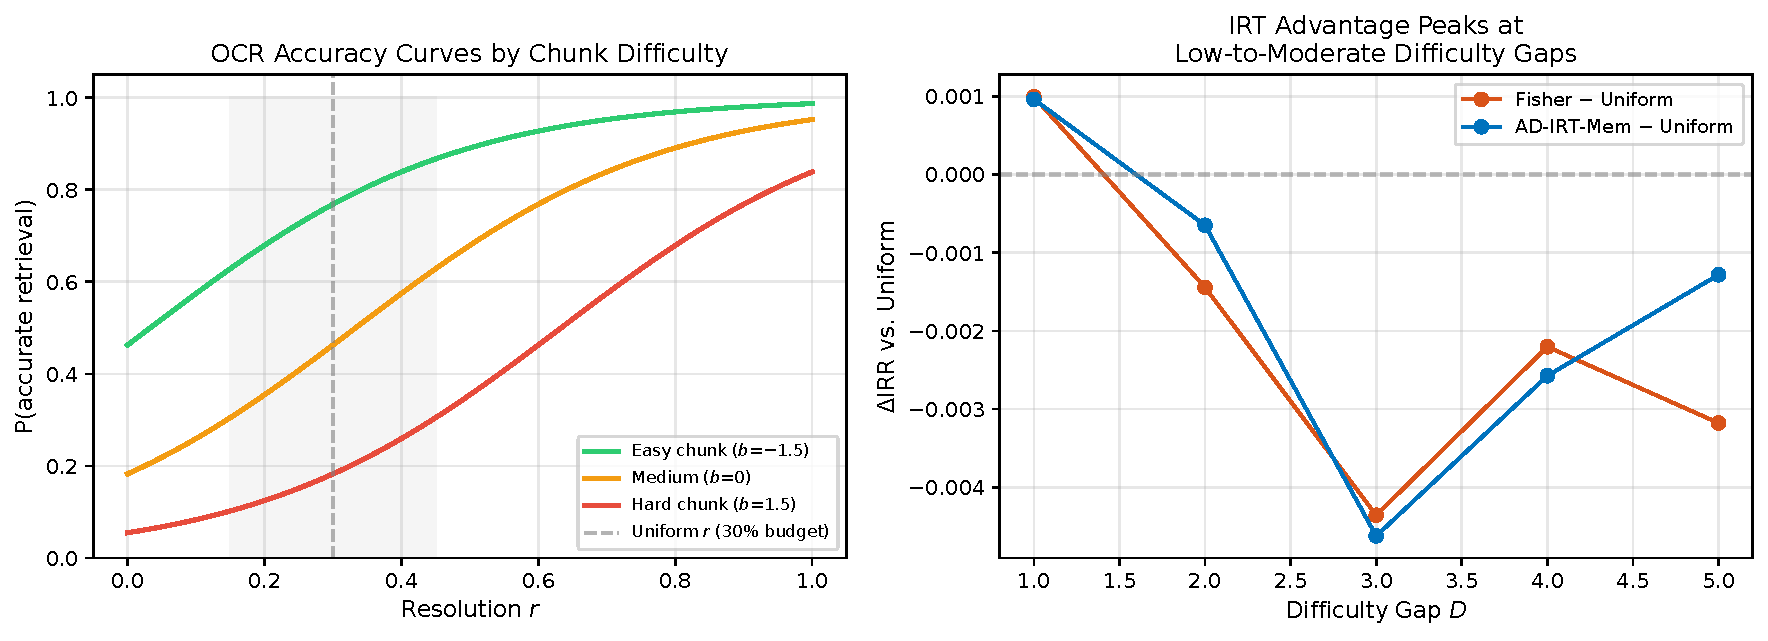
\includegraphics[width=\textwidth]{fig2_gap_interaction.pdf}
\caption{Left: OCR accuracy curves by chunk difficulty. For candidates in the concave (upper) region, marginal returns are similar, favoring uniform allocation. Right: $\Delta$IRR vs.\ uniform peaks at low difficulty gaps where some candidates span the convex region.}
\label{fig:jensen}
\end{figure}

\subsection{LLTM Feature Recovery}

Ridge regression of estimated $\hat{b}_j$ on chunk features achieves perfect weight ranking recovery ($\rho = 1.0 \pm 0.0$), with difficulty prediction $\rho = 0.446 \pm 0.007$ and in-sample $R^2 = 0.147 \pm 0.011$. The feature \emph{error density} has the highest true weight ($w = 2.0$), correctly identified as the strongest predictor.

\subsection{IRT Parameter Recovery}

Mean Spearman $\rho = 0.744$ between true and estimated chunk difficulty across all conditions, confirming that 2PL IRT extracts meaningful difficulty signals from partial historical retrieval data.

\section{Discussion}

\paragraph{The Flaw of Concentration.} EFSL~\citep{kang2026efsl} established the ``flaw of averages'' for benchmark evaluation. We identify an analogous ``flaw of concentration'' for token allocation: concentrating resolution on a few chunks (top-$k$) is catastrophic, just as evaluating only easy items inflates rankings. AD-IRT-Mem prevents this failure mode while the concavity structure of OCR accuracy keeps uniform competitive for distributed allocation.

\paragraph{When does non-uniform allocation help?} Our analysis identifies three conditions: (1)~candidate chunks span both convex and concave accuracy regions (high within-set heterogeneity); (2)~pre-filtering does not remove hard chunks entirely; (3)~budget is tight enough that allocation matters but not so tight that subset selection dominates. Current OCR-Memory pre-filtering tends to violate condition~(1) by homogenizing the candidate set.

\paragraph{Implications for OCR-Memory design.} The largest gains may come from smarter candidate selection that preserves difficulty heterogeneity, not from smarter allocation given candidates. Systems that retrieve only easy chunks eliminate the conditions under which IRT allocation helps.

\paragraph{Limitations.}
This study uses simulation only; real benchmarks such as Mind2Web~\citep{deng2023mind2web} and AppWorld~\citep{trivedi2024appworld} would strengthen evidence. Held-out query ability is approximated from historical estimates. The $w$ parameter shows high variance across conditions. The retrieval accuracy model assumes sigmoid form; real OCR accuracy may differ.

\section{Conclusion}

AD-IRT-Mem establishes a psychometric framework for OCR-Memory token allocation. The framework reveals a fundamental structural insight: the concavity of OCR accuracy functions, combined with retrieval pre-filtering, creates conditions where uniform allocation approximately equalizes marginal returns---making it hard to beat. AD-IRT-Mem's value is threefold: it prevents the top-$k$ failure mode (98.4\% win rate), provides LLTM-based cold-start difficulty estimation ($\rho = 1.0$), and identifies the precise conditions under which principled allocation can surpass uniform distribution. As OCR-Memory systems evolve, the psychometric formulation provides the theoretical foundation for adaptive allocation.

\paragraph{Code and data.} Code and data: \url{https://github.com/testofschool/ad-irt-mem}. Zenodo: \url{https://doi.org/10.5281/zenodo.20417636}

\bibliographystyle{plainnat}
\begin{thebibliography}{99}

\bibitem[Deng et~al.(2023)]{deng2023mind2web}
X.~Deng et~al. Mind2Web: Towards a generalist agent for the web. \emph{NeurIPS}, 2023.

\bibitem[Feng et~al.(2026)]{feng2026agentocr}
L.~Feng et~al. AgentOCR: Reimagining agent history via optical self-compression. \emph{arXiv:2601.04786}, 2026.

\bibitem[Fischer(1973)]{fischer1973lltm}
G.~H.~Fischer. The linear logistic test model as an instrument in educational research. \emph{Acta Psychologica}, 37:359--374, 1973.

\bibitem[Hagerman et~al.(2026)]{hagerman2026arta}
D.~Hagerman, R.~Naeem, E.~Brorsson, F.~Kahl, and L.~Svensson. ARTA: Adaptive mixed-resolution token allocation for efficient dense feature extraction. \emph{arXiv:2603.26258}, 2026.

\bibitem[Kang(2026a)]{kang2026efsl}
J.~M.~Kang. The scaling law of evaluation failure. \emph{arXiv:2605.11205}, 2026.

\bibitem[Kang(2026b)]{kang2026adirt}
J.~M.~Kang. AD-IRT: Adaptive dimensionality IRT for sparse cross-benchmark evaluation. Companion manuscript, 2026.

\bibitem[Kang(2026c)]{kang2026pcr}
J.~M.~Kang. Psychometric content routing. Companion manuscript, 2026.

\bibitem[Li et~al.(2026)]{li2026ocr}
J.~Li et~al. OCR-Memory: Optical context retrieval for long-horizon agent memory. \emph{arXiv:2604.26622}, 2026.

\bibitem[Lord and Novick(1968)]{lord1968statistical}
F.~M.~Lord and M.~R.~Novick. \emph{Statistical Theories of Mental Test Scores}. Addison-Wesley, 1968.

\bibitem[Shi et~al.(2026)]{shi2026memocr}
Y.~Shi et~al. MemOCR: Layout-aware visual memory for efficient long-horizon reasoning. \emph{arXiv:2601.21468}, 2026.

\bibitem[Song et~al.(2025)]{song2025irt}
W.~Song et~al. IRT-Router: Effective and interpretable multi-LLM routing via item response theory. \emph{Proc.\ ACL}, 2025.

\bibitem[Trivedi et~al.(2024)]{trivedi2024appworld}
H.~Trivedi et~al. AppWorld: A controllable world of apps and people for benchmarking interactive coding agents. \emph{arXiv:2407.18901}, 2024.

\bibitem[Wei et~al.(2025)]{wei2025deepseekocr}
H.~Wei et~al. DeepSeek-OCR: Contexts optical compression. \emph{arXiv:2510.18234}, 2025.

\end{thebibliography}

\appendix
\section{Sparsity Analysis}
\begin{figure}[ht!]
\centering
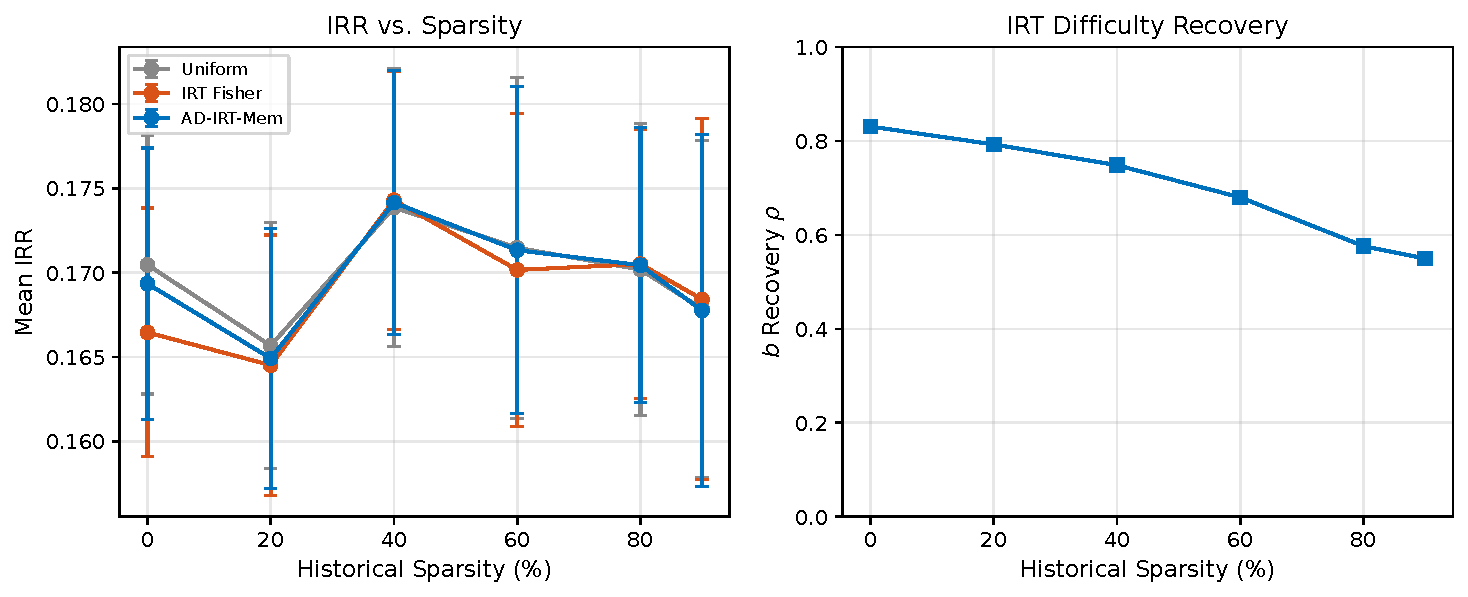
\includegraphics[width=0.9\textwidth]{fig3_sparsity.pdf}
\caption{Left: IRR remains broadly similar across methods and sparsity levels. Right: IRT difficulty recovery $\rho$ degrades with sparsity, as expected.}
\label{fig:sp}
\end{figure}

\end{document}
